\chapter{Analysis of 30-Day Spending and Consumption Patterns}

I tracked every personal transaction from May~7 to June~4, 2026---67 transactions exported from my ABBank app. Major household costs (apartment fees, electricity, water) are paid by my family and excluded. The data covers only the spending I personally control.

\section{Spending Summary by Category}

\begin{table}[h!]
\caption{30-Day Personal Spending Breakdown}
\label{tab:spending_breakdown}
\begin{tabularx}{\linewidth}{@{}lrrL@{}}
\toprule
\textbf{Category} & \textbf{Total (VND)} & \textbf{Share (\%)} & \textbf{Key Drivers} \\
\midrule
Food            & 3,810,866 & 73.4\% & Dining out, social gatherings, groceries \\
Sports          &   759,000 & 14.6\% & Badminton court bookings, racket restringing \\
Shopping online &   474,999 &  9.2\% & Phone cards, e-commerce purchases \\
Entertainment   &   145,000 &  2.8\% & Gaming cafes, digital subscriptions \\
\midrule
\textbf{Total}  & \textbf{5,189,865} & \textbf{100.0\%} & \\
\bottomrule
\end{tabularx}
\end{table}

\section{Consumption Pattern Analysis}

\begin{wrapfigure}{r}{0.42\textwidth}
  \vspace{-10pt}
  \centering
  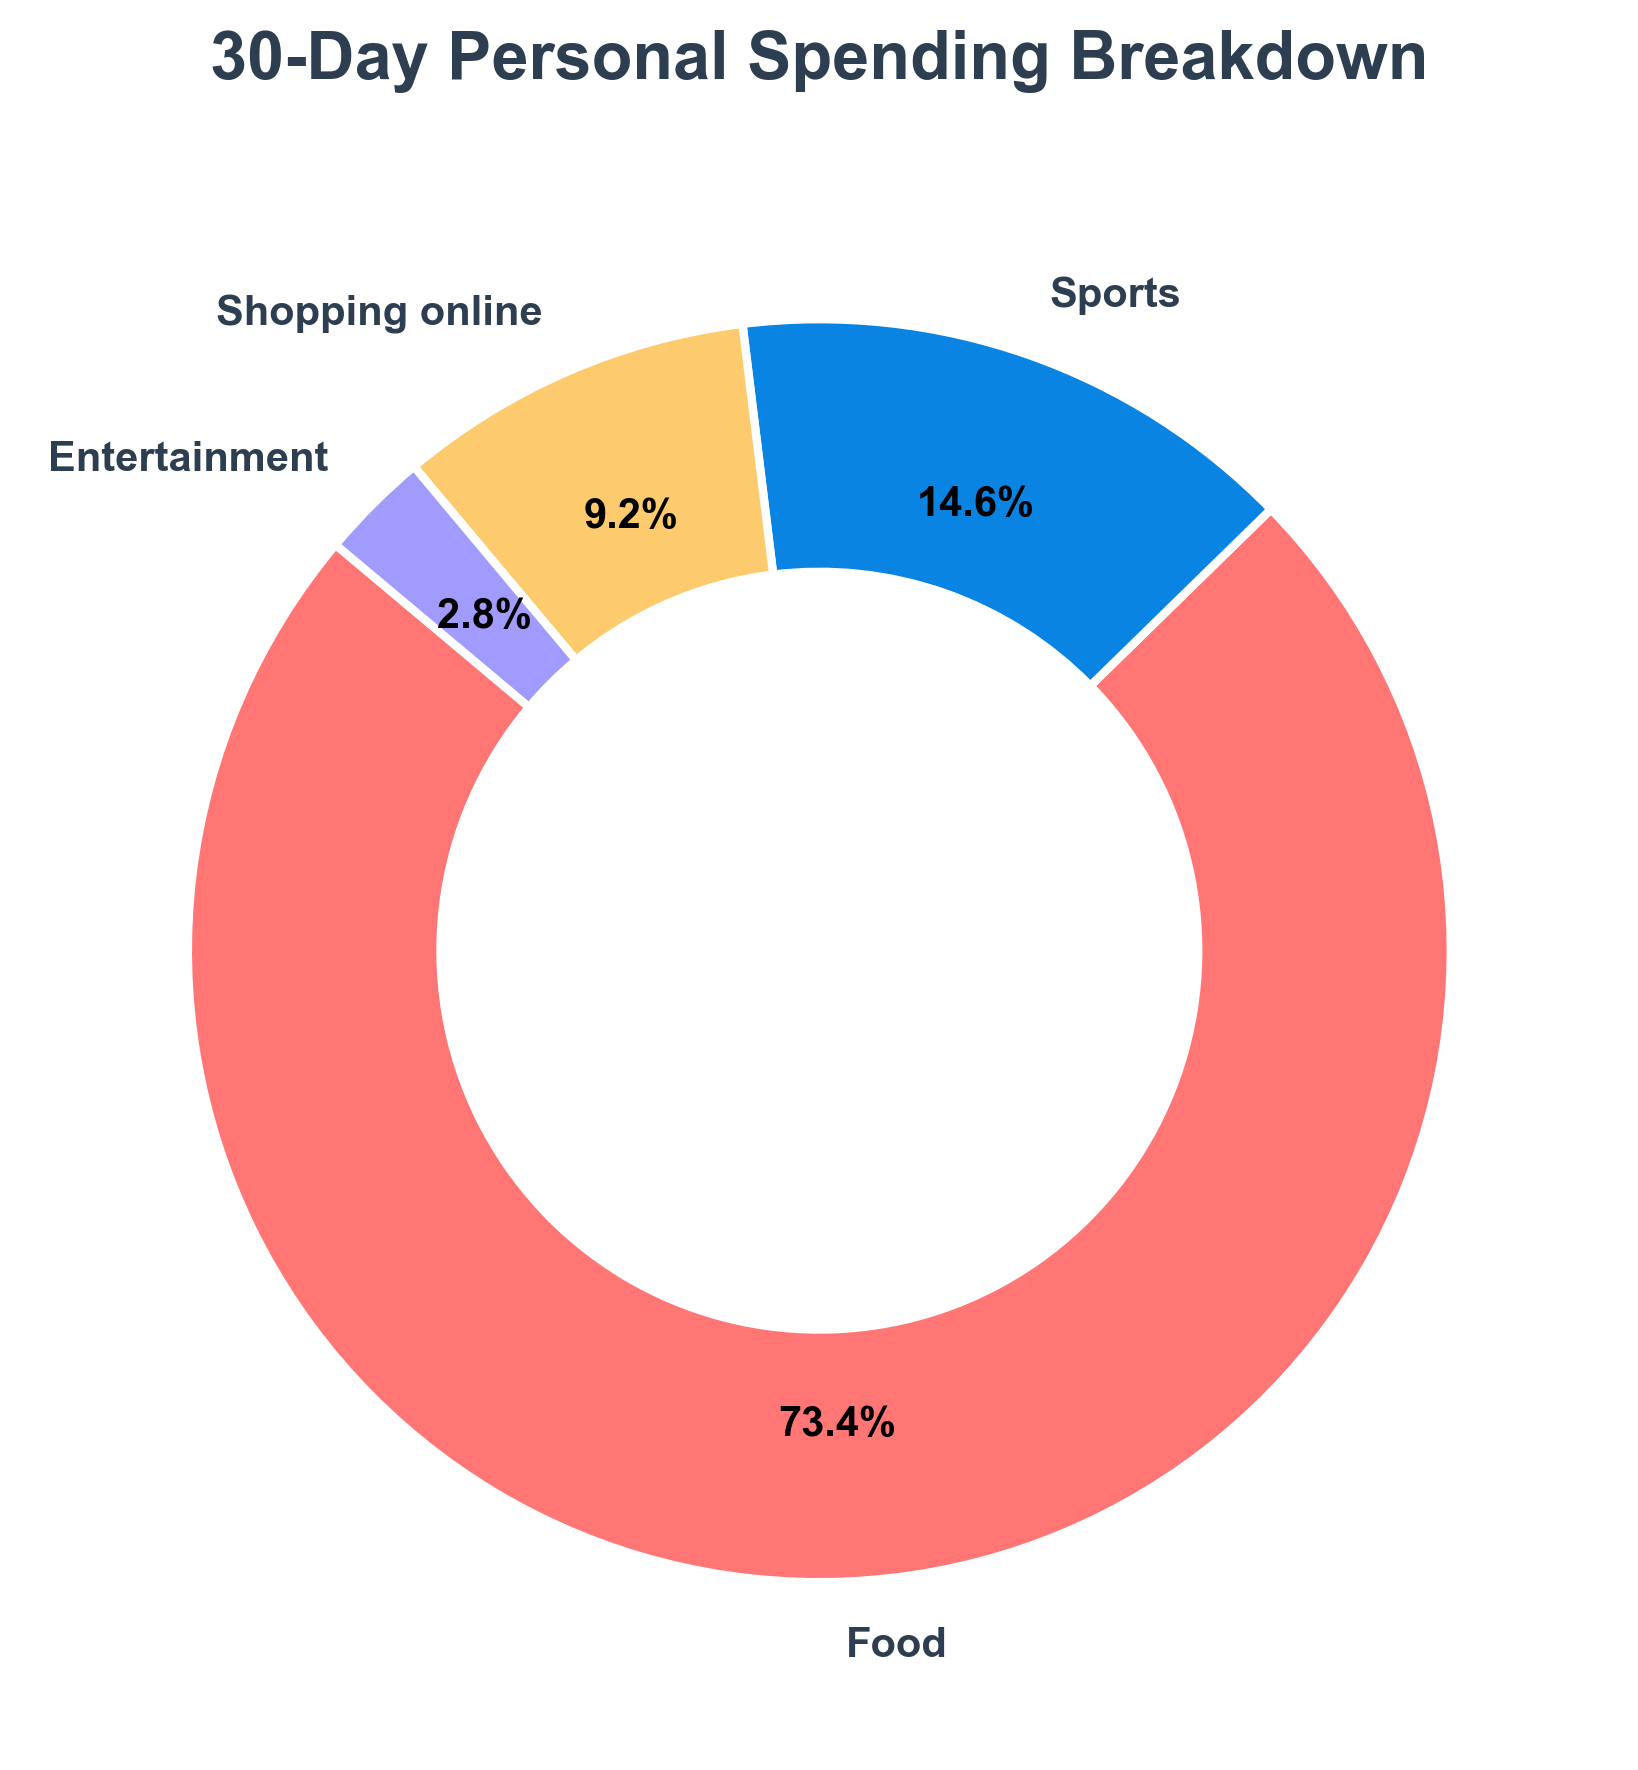
\includegraphics[width=0.40\textwidth]{figures/spending_pie.png}
  \caption{30-day spending by category}
  \label{fig:spending_pie}
  \vspace{-8pt}
\end{wrapfigure}

Food dominates at 73.4\% (3,810,866~VND), split between necessary home groceries from WinCommerce and discretionary dining out and social ``nhậu'' sessions. The discretionary share is the target for reduction. Sports spending at 14.6\% (759,000~VND) covers badminton court bookings and Exbolt~63 restringing at 220,000~VND every two weeks---treated as a committed health cost, not a luxury. Online shopping and entertainment combined account for 12.0\% and are already low, reflecting consistent restraint on non-essential purchases.

\section{Strategic Adjustments}

Two adjustments follow from the data. First, cut dining-out by 30\%---fewer restaurant meals and social drinking sessions, more home cooking. This alone is projected to save over 810,000~VND per month, or 9,700,000~VND per year. Second, share badminton court costs consistently with regular play partners to reduce the per-person sports expense without cutting back on physical activity.

Of the two, the food reduction is the more behaviorally demanding. A large share of the discretionary food spend is tied to social occasions---meals with friends, after-work ``nhậu'' sessions, group outings. These are not purely wasteful; they have real social value. The 30\% target is calibrated to reduce frequency without cutting them out entirely: cooking at home on weekday evenings, treating dining out as a deliberate choice rather than a default, and being more selective about which social occasions are worth the spend. The savings potential is the highest of any category in the budget, and it requires no income increase to realize.
